

\chapter{Data Manipulation Language e Data Query Language}
\label{cap:dml_dql}

\section{Atividade Prática: Modelagem de Dados}

\begin{tcolorbox}[colback=green!5,colframe=green!40!black,title=Exercício Dirigido com o Professor]
Nesta etapa, realizaremos a modelagem lógica da nossa primeira entidade. Sob a orientação do professor, analise os atributos necessários para representar uma \textbf{Pessoa} no sistema. 

O objetivo é compreender como as regras de negócio do mundo real se transformam em restrições (\textit{constraints}) no PostgreSQL.
\end{tcolorbox}

\subsection{Estrutura Lógica da Tabela \texttt{pessoa}}

Abaixo, detalhamos a estrutura que será implementada. Preste atenção aos tipos de dados e às propriedades de cada campo:

\begin{itemize}
    \item \textbf{id}: Chave Primária (\textit{Primary Key}). Será do tipo \texttt{SERIAL} para garantir que o identificador seja autoincrementado e exclusivo.
    \item \textbf{nome}: Nome completo. Campo \textbf{obrigatório} (\textit{NOT NULL}), definido como \texttt{VARCHAR(100)}.
    \item \textbf{cpf}: Cadastro de Pessoa Física. Deve ser \textbf{único} (\textit{UNIQUE}) e \textbf{obrigatório}, garantindo que não haja duplicidade de registros.
    \item \textbf{email}: Endereço eletrônico. Também deve ser \textbf{único}, permitindo o uso como login ou canal de comunicação exclusivo.
    \item \textbf{data\_nascimento}: Campo do tipo \texttt{DATE}, essencial para o cálculo de idade e validações de maioridade.
    \item \textbf{criado\_em}: Registro automático de auditoria. Armazena a data e hora exata em que o registro foi inserido no banco.
\end{itemize}



\vspace{0.5cm}
\begin{center}
\textit{\textbf{Nota para o aluno:} Durante a explicação do professor, anote quais desses campos poderiam ser opcionais em um cenário real e quais devem ser sempre protegidos por restrições de integridade.}
\end{center}

\begin{figure}[H]
     \centering
     \begin{subfigure}[b]{0.45\textwidth}
         \centering
         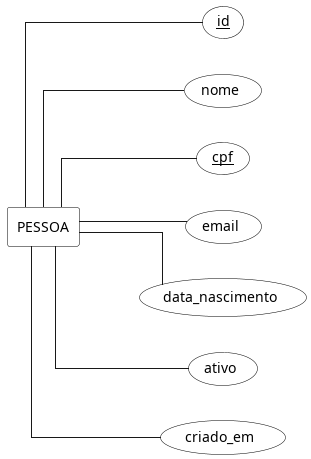
\includegraphics[width=\textwidth]{Pessoa_ER.png}
         \caption{Diagrama ER}
         \label{fig:atributosER}
     \end{subfigure}
     \hfill
     \begin{subfigure}[b]{0.45\textwidth}
         \centering
         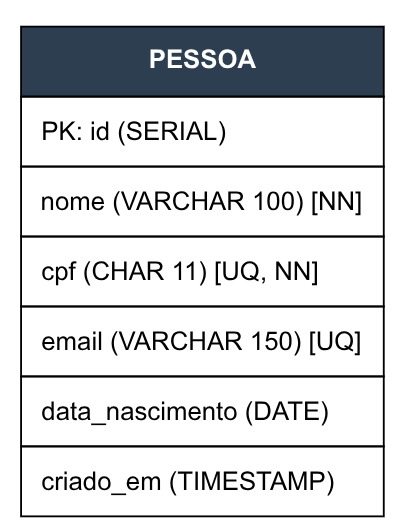
\includegraphics[width=\textwidth]{PessoaLogico.png}
         \caption{Diagrama Lógico}
         \label{fig:atributos_logico}
     \end{subfigure}
     \caption{Modelagem da Entidade Pessoa: Visão ER e Lógica.}
     \label{fig:modelagem_pessoa}
\end{figure}
\section{Script SQL de Criação}

O código abaixo executa a criação da tabela no schema \texttt{public}.

\begin{sqlcode}
CREATE TABLE pessoa (
    id SERIAL PRIMARY KEY,
    nome VARCHAR(100) NOT NULL,
    cpf CHAR(11) UNIQUE NOT NULL,
    email VARCHAR(150) UNIQUE,
    data_nascimento DATE,
    ativo BOOLEAN DEFAULT TRUE,
    criado_em TIMESTAMP WITH TIME ZONE DEFAULT CURRENT_TIMESTAMP
);

-- Adicionar um comentário na tabela para documentação

COMMENT ON TABLE pessoa IS 'Tabela que armazena dados cadastrais de pessoas físicas';
\end{sqlcode}

\section{Operações Básicas (DML)}

\subsection{Inserção de Dados}
Para inserir um novo registro, utilize o comando abaixo:

\begin{sqlcode}
INSERT INTO pessoa (nome, cpf, email, data_nascimento) 
VALUES ('João Silva', '12345678901', 'joao@email.com', '1990-05-15');
\end{sqlcode}

\subsection{Consulta}
Para listar todas as pessoas cadastradas:

\begin{sqlcode}
SELECT id, nome, email FROM pessoa WHERE ativo = TRUE;
\end{sqlcode}
\begin{figure}[H]
    \centering
    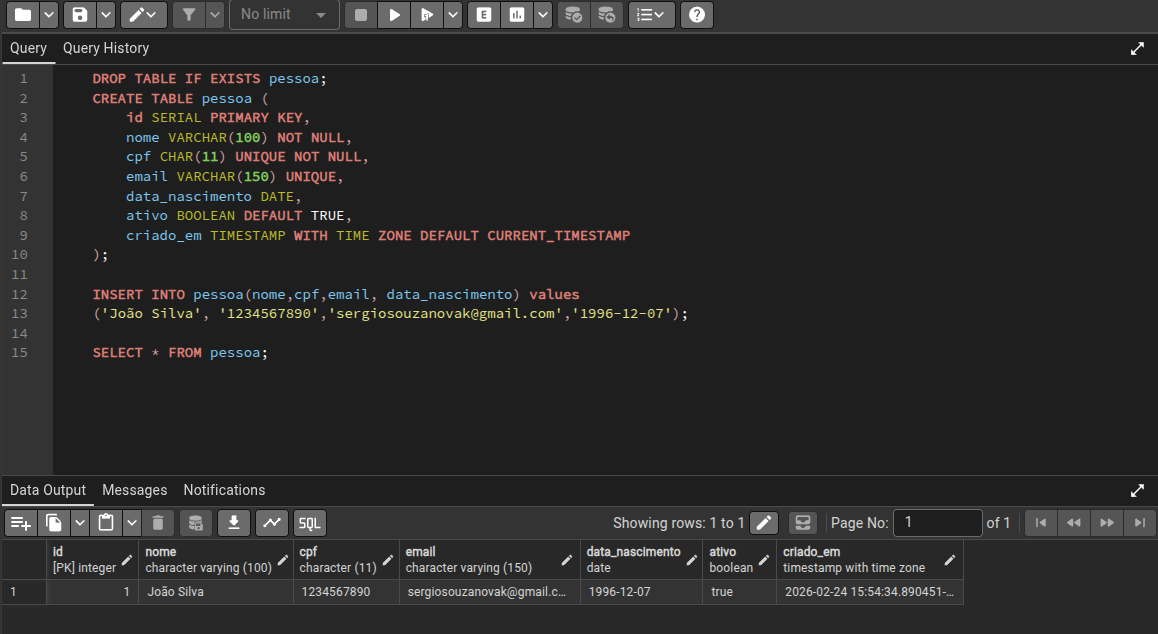
\includegraphics[width=15.3cm]{execucao_select_primeira_tabela.png}
    \caption{Execução do comando SELECT na tabela pessoa.}
    \label{fig:execucao_select_pessoa}
\end{figure}


\section{Comando SELECT: Estrutura e Funcionalidades}

\begin{sqlcode}
SELECT nome, salario
FROM funcionarios
WHERE salario > 30020
ORDER BY salario DESC; 
\end{sqlcode}

O comando \texttt{SELECT} é utilizado para realizar consultas em um banco de dados relacional. Sua principal finalidade é recuperar dados armazenados em uma ou mais tabelas, permitindo ao usuário visualizar informações específicas conforme determinados critérios.

A estrutura básica do comando é:

\begin{sqlcode}
SELECT coluna1, coluna2, ...
FROM nome_da_tabela;
\end{sqlcode}

Nesse formato, especificam-se as colunas que se deseja visualizar após a palavra-chave \texttt{SELECT}, enquanto a cláusula \texttt{FROM} indica a tabela de onde os dados serão obtidos. Caso seja necessário retornar todas as colunas da tabela, pode-se utilizar o caractere curinga \texttt{*}, como no exemplo:

\begin{sqlcode}
SELECT * FROM alunos;
\end{sqlcode}

Além disso, o comando \texttt{SELECT} pode ser combinado com outras cláusulas para refinar a consulta. Entre as mais utilizadas estão:

\begin{itemize}
    \item \texttt{WHERE}: filtra registros de acordo com uma condição lógica;
    \item \texttt{ORDER BY}: organiza os resultados em ordem crescente ou decrescente;
    \item \texttt{GROUP BY}: agrupa registros para aplicação de funções agregadas;
    \item \texttt{HAVING}: define condições sobre grupos;
    \item \texttt{LIMIT}: restringe a quantidade de registros retornados (em alguns SGBDs).
\end{itemize}

Por exemplo:

\begin{sqlcode}
SELECT nome, idade
FROM alunos
WHERE idade > 18
ORDER BY idade DESC;
\end{sqlcode}

Nesse caso, a consulta retorna apenas os alunos com idade superior a 18 anos, organizando o resultado em ordem decrescente de idade.Portanto, o comando \texttt{SELECT} é a base das operações de consulta em SQL, sendo essencial para a extração e análise de dados em sistemas de gerenciamento de bancos de dados relacionais.

\subsection{Praticando Filtros e Ordenação: WHERE e ORDER BY}

\begin{tcolorbox}[colback=blue!5,colframe=blue!40!black,title=Exercício Dirigido com o Professor: Refinando a Busca]
Em sistemas reais, um banco de dados pode conter milhões de registros. Retornar todos os dados de uma vez não é apenas ineficiente, mas muitas vezes inútil para o usuário final. Sob a orientação do professor, vamos testar na nossa tabela \texttt{Pessoa} como extrair apenas a informação exata que precisamos.
\end{tcolorbox}

\subsection{A Cláusula \texttt{WHERE} (Onde)}

A cláusula \texttt{WHERE} atua como um "peneira". Ela avalia cada linha da tabela e retorna apenas aquelas que satisfazem uma condição lógica. Podemos usar operadores de comparação como \texttt{=}, \texttt{>}, \texttt{<}, \texttt{>=}, \texttt{<=} e \texttt{<>} (diferente).



Por exemplo, se quisermos encontrar apenas os usuários que estão com o cadastro ativo em nosso sistema:

\begin{sqlcode}
-- O banco de dados retornará apenas as linhas onde 'ativo' for verdadeiro
SELECT nome, email 
FROM pessoa 
WHERE ativo = TRUE;
\end{sqlcode}

Outro exemplo comum é o uso com datas. Vamos buscar todas as pessoas que nasceram após o ano 2000:

\begin{sqlcode}
SELECT nome, data_nascimento 
FROM pessoa 
WHERE data_nascimento > '2000-12-31';
\end{sqlcode}

\subsection{A Cláusula \texttt{ORDER BY} (Ordenar Por)}

Enquanto o \texttt{WHERE} decide \textit{quais} linhas serão exibidas, o \texttt{ORDER BY} decide \textit{em qual ordem} elas aparecerão na tela. A ordenação pode ser feita em duas direções:

\begin{itemize}
    \item \textbf{\texttt{ASC}} (Ascendente): Ordem crescente (A-Z, 0-9, datas mais antigas para as mais recentes). Se você não especificar a direção, o SQL usará \texttt{ASC} por padrão.
    \item \textbf{\texttt{DESC}} (Descendente): Ordem decrescente (Z-A, 9-0, datas mais recentes para as mais antigas).
\end{itemize}
Se o professor pedir para organizar a lista de pessoas em ordem alfabética inversa (de Z a A), o comando será:
\begin{sqlcode}
SELECT nome, cpf 
FROM pessoa 
ORDER BY nome DESC;
\end{sqlcode}

\subsubsection{Juntando as Peças}

O verdadeiro poder do SQL aparece quando combinamos essas cláusulas. É importante notar que \textbf{a ordem dos comandos importa}: o \texttt{WHERE} sempre deve vir antes do \texttt{ORDER BY}.

Vamos resolver um cenário prático: \textit{"Liste o nome e a data de nascimento de todas as pessoas com cadastro ativo, ordenando das mais velhas para as mais novas"}.

\begin{sqlcode}
SELECT nome, data_nascimento
FROM pessoa
WHERE ativo = TRUE
ORDER BY data_nascimento ASC;
\end{sqlcode}


\subsection{Restringindo e Agrupando Resultados: LIMIT e HAVING}

\begin{tcolorbox}[colback=blue!5,colframe=blue!40!black,title=Exercício Dirigido com o Professor: Top Resultados e Agrupamentos]
À medida que nosso banco de dados cresce, algumas perguntas mudam. Em vez de perguntar "Quais são todos os usuários?", passamos a perguntar "Quais são os 5 usuários mais recentes?" ou "Quantos usuários ativos temos em comparação aos inativos?". Acompanhe com o professor como responder a essas perguntas de negócios.
\end{tcolorbox}

\subsubsection{A Cláusula \texttt{LIMIT} (Limite de Linhas)}

A cláusula \texttt{LIMIT} é extremamente útil para \textbf{paginação} (como quando você avança para a "página 2" de uma pesquisa no Google) ou para buscar os resultados do "Top N" (os maiores, menores, mais recentes, etc.). Ela simplesmente corta o resultado final para exibir apenas a quantidade de linhas especificada.


\textbf{Exemplo Prático:} Se o professor pedir para listar apenas as \textbf{3 pessoas cadastradas mais recentemente}, precisamos ordenar pela data de criação de forma decrescente e, em seguida, aplicar o limite:

\begin{sqlcode}
-- Traz os 3 registros mais novos
SELECT nome, criado_em
FROM pessoa
ORDER BY criado_em DESC
LIMIT 3;
\end{sqlcode}

\subsubsection{A Cláusula \texttt{HAVING} (Filtro de Grupos)}

Para entender o \texttt{HAVING}, primeiro precisamos lembrar do \texttt{GROUP BY} (Agrupar Por), que une registros que possuem valores idênticos em uma ou mais colunas, permitindo o uso de funções matemáticas como \texttt{COUNT()} (contar), \texttt{SUM()} (somar) ou \texttt{AVG()} (média).

A grande confusão dos alunos iniciantes é: \textit{Qual a diferença entre WHERE e HAVING?}
\begin{itemize}
    \item O \textbf{\texttt{WHERE}} filtra \textbf{linhas individuais} ANTES de serem agrupadas.
    \item O \textbf{\texttt{HAVING}} filtra \textbf{os grupos} DEPOIS que eles foram formados.
\end{itemize}

\textbf{Exemplo Prático:} Vamos agrupar as pessoas pelo status (\texttt{ativo} = \texttt{TRUE} ou \texttt{FALSE}) e contar quantas pessoas existem em cada grupo. Porém, o professor solicitou que a consulta mostre \textbf{apenas os grupos que possuam mais de 10 pessoas}. 

Como a restrição "mais de 10" é baseada no resultado de uma contagem (um grupo), \textbf{não podemos usar o WHERE}. Usamos o \texttt{HAVING}:

\begin{sqlcode}
SELECT ativo, COUNT(id) AS total_pessoas
FROM pessoa
GROUP BY ativo
HAVING COUNT(id) > 10;
\end{sqlcode}

\vspace{0.5cm}
\begin{tcolorbox}[colback=red!5,colframe=red!70!black,title=Atenção à Ordem de Execução!]
O banco de dados SQL segue uma ordem estrita para ler o seu comando. Se você for usar todas as cláusulas que aprendemos até agora em uma única consulta, a ordem \textbf{obrigatória} no código deve ser:
\begin{enumerate}
    \item \texttt{SELECT} (O que mostrar)
    \item \texttt{FROM} (De qual tabela)
    \item \texttt{WHERE} (Filtro de linhas)
    \item \texttt{GROUP BY} (Como agrupar)
    \item \texttt{HAVING} (Filtro de grupos)
    \item \texttt{ORDER BY} (Ordem de exibição final)
    \item \texttt{LIMIT} (Quantidade final de linhas)
\end{enumerate}
\end{tcolorbox}



\section{Estudo Dirigido: Agrupamentos e a Cláusula \texttt{HAVING}}

\begin{tcolorbox}[colback=green!5,colframe=green!40!black,title=Objetivo da Atividade]
Neste exercício, vamos simular um sistema de vendas para entender como o SQL pode realizar cálculos complexos e filtrar resultados baseados em agregados (somas), algo que o \texttt{WHERE} não consegue fazer sozinho.
\end{tcolorbox}

\subsection{Passo 1: Criando o Cenário de Teste}

O primeiro passo é criar uma tabela temporária. Tabelas do tipo \texttt{TEMP} existem apenas durante a sua sessão atual no banco de dados.

\begin{sqlcode}
-- 1. Criar tabela de vendas rápida
CREATE TEMP TABLE vendas (
    id SERIAL,
    produto VARCHAR(50),
    categoria VARCHAR(50),
    valor DECIMAL(10,2)
);
\end{sqlcode}

\subsection{Passo 2: Populando a Tabela}

Vamos inserir dados que nos permitam comparar categorias diferentes. Observe que a categoria 'Eletrônicos' terá um valor total maior que 'Papelaria'.

\begin{sqlcode}
-- 2. Inserir dados para teste
INSERT INTO vendas (produto, categoria, valor) VALUES
('Teclado', 'Eletrônicos', 80.00),
('Mouse',   'Eletrônicos', 50.00),  -- Soma Eletrônicos: 130.00
('Caderno', 'Papelaria',   15.00),
('Caneta',  'Papelaria',    5.00);  -- Soma Papelaria: 20.00
\end{sqlcode}

\subsection{Passo 3: A Consulta de Faturamento}



Agora, execute a query abaixo. O objetivo é listar o faturamento total por categoria, mas \textbf{excluir} do relatório qualquer categoria que tenha vendido menos de 100.00 no total.

\begin{sqlcode}
-- 3. Testar a query com HAVING
SELECT categoria, SUM(valor) AS faturamento_total
FROM vendas
GROUP BY categoria
HAVING SUM(valor) > 100.00;
\end{sqlcode}

\begin{tcolorbox}[colback=orange!5,colframe=orange!75!black,title=Questionário de Reflexão]
Após executar os comandos acima, discuta com o professor:
\begin{enumerate}
    \item Por que a categoria 'Papelaria' não apareceu no resultado final?
    \item Se mudarmos o valor do \texttt{HAVING} para \texttt{10.00}, o que acontece?
    \item Tente substituir \texttt{HAVING SUM(valor) > 100.00} por \texttt{WHERE SUM(valor) > 100.00}. Qual erro o PostgreSQL retorna? Por que isso acontece?
\end{enumerate}
\end{tcolorbox}

\subsection{Diferença Crucial: WHERE vs HAVING}

Para nunca mais esquecer:
\begin{itemize}
    \item \textbf{WHERE}: Filtra os dados \textbf{antes} da soma (ex: excluir o produto 'Caneta' antes de somar).
    \item \textbf{HAVING}: Filtra os dados \textbf{depois} da soma (ex: olhar o total da categoria e decidir se mostra ou não).
\end{itemize}

\section{Análise Avançada: Funções de Agregação e Comportamento do Agrupamento}

Nesta etapa do estudo dirigido, vamos analisar como o banco de dados se comporta quando alteramos a lógica da nossa "pergunta". O código abaixo prepara uma base com diferentes estados de atividade para testarmos a sensibilidade das funções \texttt{COUNT} e \texttt{SUM}.

\subsection{Script de Preparação}

Observe que estamos lidando com restrições de integridade (\textit{Unique}) e valores padrão (\textit{Default}).

\begin{sqlcode}
DROP TABLE IF EXISTS PESSOA;

CREATE TABLE PESSOA (
    ID SERIAL PRIMARY KEY,
    NOME VARCHAR(100) NOT NULL,
    CPF CHAR(11) UNIQUE NOT NULL,
    EMAIL VARCHAR(150) UNIQUE,
    DATA_NASCIMENTO DATE,
    ATIVO BOOLEAN DEFAULT TRUE,
    CRIADO_EM TIMESTAMP WITH TIME ZONE DEFAULT CURRENT_TIMESTAMP
);

-- Inserindo dois registros inativos
INSERT INTO PESSOA (NOME, CPF, EMAIL, DATA_NASCIMENTO, ATIVO)
VALUES ('João Silva', '12345678900', 'joao@email.com', '1996-12-07', false),
       ('Camila Santana', '12345678901', 'camila@email.com', '1996-12-07', false);

-- Inserindo um registro ativo (padrão)
INSERT INTO PESSOA (NOME, CPF, EMAIL, DATA_NASCIMENTO)
VALUES ('João Silv1a', '12345678902', 'joao2@email.com', '1996-12-07');
\end{sqlcode}

\subsection{Discussão: COUNT vs SUM}

A consulta original utiliza a função \texttt{COUNT(ID)}. Mas o que aconteceria se tentássemos usar \texttt{SUM}?



\begin{sqlcode}
-- Consulta A: Contagem por grupo
SELECT ATIVO, COUNT(ID) AS TOTAL_PESSOAS 
FROM PESSOA 
GROUP BY ATIVO;
\end{sqlcode}

\begin{tcolorbox}[colback=red!5,colframe=red!75!black,title=Conceito Fundamental]
\begin{itemize}
    \item \textbf{COUNT(ID)}: Conta quantas \textbf{linhas} existem no grupo. Funciona com qualquer tipo de dado (números, texto, datas, booleanos). No nosso exemplo, resultará em 2 para \textit{false} e 1 para \textit{true}.
    \item \textbf{SUM(coluna)}: Tenta realizar uma \textbf{adição aritmética} dos valores. Só funciona com tipos de dados numéricos (inteiros, decimais).
\end{itemize}
\end{tcolorbox}

\subsection{O que acontece se alterarmos para SUM?}

Se tentarmos rodar \texttt{SELECT ATIVO, SUM(ID) FROM PESSOA GROUP BY ATIVO;}, o banco somará os valores numéricos das Chaves Primárias.

\begin{table}[H]
    \centering
    \begin{tabular}{|l|l|l|}
    \hline
    \textbf{Função} & \textbf{Lógica} & \textbf{Resultado (para ATIVO = false)} \\ \hline
    \texttt{COUNT(ID)} & 1 + 1 (duas ocorrências) & \textbf{2} \\ \hline
    \texttt{SUM(ID)} & ID 1 + ID 2 (soma dos valores) & \textbf{3} \\ \hline
    \end{tabular}
    \caption{Diferença de resultado entre contar e somar.}
\end{table}



\begin{tcolorbox}[colback=orange!5,colframe=orange!70!black,title=Reflexão para o Aluno]
\textbf{Pergunta:} Por que não poderíamos usar \texttt{SUM(NOME)}?
\end{tcolorbox}


\section{Inserção de Dados: O Comando \texttt{INSERT INTO}}

Após criar a estrutura das tabelas com o \texttt{CREATE TABLE}, o próximo passo é popular o banco de dados. O comando \texttt{INSERT} é utilizado para inserir novos registros (linhas) em uma tabela existente.



\subsection{Sintaxe Básica}

Existem duas formas principais de utilizar este comando. A mais segura e recomendada é especificar explicitamente as colunas onde os dados serão inseridos:

\begin{sqlcode}
INSERT INTO nome_da_tabela (coluna1, coluna2, ...)
VALUES (valor1, valor2, ...);
\end{sqlcode}

\subsection{Regras Cruciais para Inserção}

Para que a inserção ocorra sem erros, o desenvolvedor deve seguir algumas regras fundamentais de sintaxe e integridade:

\begin{itemize}
    \item \textbf{Textos e Datas}: Devem sempre estar entre aspas simples (ex: \texttt{'João Silva'}, \texttt{'2024-05-10'}).
    \item \textbf{Números}: Não utilizam aspas (ex: \texttt{1500.50}, \texttt{25}).
    \item \textbf{Ordem}: A ordem dos valores no \texttt{VALUES} deve ser exatamente a mesma das colunas listadas.
    \item \textbf{Campos Obrigatórios}: Colunas com a restrição \texttt{NOT NULL} devem obrigatoriamente receber um valor, a menos que possuam um \texttt{DEFAULT}.
\end{itemize}

\subsection{Prática: Inserindo Dados na Tabela Pessoa}

Vamos aplicar o comando à tabela que modelamos anteriormente. Observe que não precisamos inserir o campo \texttt{ID}, pois ele é do tipo \texttt{SERIAL} e o banco o gera automaticamente.

\begin{sqlcode}
-- Insercao especificando as colunas
INSERT INTO pessoa (nome, cpf, email, data_nascimento)
VALUES ('Ana Souza', '12345678910', 'ana@email.com', '1992-08-24');

-- Insercao de multiplos registros em um unico comando
INSERT INTO pessoa (nome, cpf, email)
VALUES 
    ('Carlos Luz', '98765432100', 'carlos@email.com'),
    ('Beatriz Vaz', '55544433322', 'beatriz@email.com');
\end{sqlcode}



\begin{tcolorbox}[colback=red!5,colframe=red!40!black,title=Atenção: Erros de Restrição]
Se você tentar inserir um CPF que já existe ou deixar de preencher um campo \texttt{NOT NULL}, o PostgreSQL impedirá a operação e retornará um erro de \textbf{violação de restrição}. Isso garante que o banco de dados nunca aceite dados inválidos ou "sujos".
\end{tcolorbox}

\begin{tcolorbox}[colback=blue!5,colframe=blue!40!black,title=Dica do Professor: Omissions]
Campos que possuem \texttt{DEFAULT} (como o campo \texttt{ativo} ou \texttt{criado\_em} da nossa tabela) podem ser omitidos no \texttt{INSERT}. O PostgreSQL preencherá automaticamente com o valor padrão definido na criação da tabela.
\end{tcolorbox}

\vspace{0.5cm}
\begin{center}

\end{center}


% \begin{observacao}
% Observe que usamos \texttt{ORDER BY} para ordenar os resultados de forma decrescente.
% \end{observacao}

% \section{Exercício}
% Crie uma tabela de clientes com os campos \texttt{id}, \texttt{nome} e \texttt{email}.

% \begin{sqlcode}
% CREATE TABLE clientes (
%     id INT PRIMARY KEY,
%     nome VARCHAR(100) NOT NULL,
%     email VARCHAR(150) UNIQUE
% );
% \end{sqlcode}